\documentclass{article}
\usepackage{graphicx}
\newcommand{\documentname}{paper~}
\newcommand{\match}{{\tt match}~}
\newcommand{\apj}{ApJ}
\newcommand{\apjs}{ApJS}
\newcommand{\apjl}{ApJL}
\newcommand{\aj}{AJ}
\newcommand{\mnras}{MNRAS}
\newcommand{\mnrassub}{MNRAS accepted}
\newcommand{\aap}{A\&A}
\newcommand{\aaps}{A\&AS}
\newcommand{\araa}{ARA\&A}
\newcommand{\nat}{Nature}
\newcommand{\physrep}{PhR}
\newcommand{\pasp}{PASP}
\newcommand{\pasj}{PASJ}
\newcommand{\hMpc}{{\ifmmode{h^{-1}{\rm Mpc}}\else{$h^{-1}$Mpc }\fi}} 
\title{Non-local effects of matter discreteness and inhomogeneity on
  cosmic flows}  \author{Jaime E. Forero-Romero}
\begin{document}
\maketitle
\begin{abstract}

Gravity is the dominant force shaping the spatial distribution of galaxies in
the Universe on its largest scales. Under the assumption of
homogeneity and isotropy one could approximate the local
kinematic evolution by the near matter distribution below an
homogeneity scale. In this letter we show that if the matter
distribution is composed by a discrete set of points then, due to
statistical fluctuations, the gravitational influence does not have a
cut down scale. Our results are based on straightforward
analytical considerations, monte-carlo realizations and cosmological
N-body simulations. We discuss the implications of these results in
the interpretation of the peculiar motion of our galaxy and bulk
galaxy flows in the local universe. We also suggest new cosmological
tests of these ideas. 



\end{abstract}

The gravitational force plays the dominant role in
defining the large scale structure of the Universe. Starting from very
homogeneous conditions in the matter distribution, gravity drives the emergence
of a web-like pattern in the distribution of galaxies. The influence of
far away matter can be discarded on the grounds that the net
gravitational force inside an homogeneous spherical shell is zero. In
classical newtonian mechanics it is possible to show that the net
force inside an homogeneous and continus shell of matter is exactly
zero. The same is valid in general relativity. That result receives
the name of the Birkhoff's theorem.  

The observational advances in the last two decades have allowed us
to measure the distribution of galaxies on very large scales. The
spatial pattern they follow is highly structured. It resembles a
large network of interconnected filaments and sheets crossing large
underdense regions.  This is why the community referes to this
structure as the cosmic web. At the same time the concept of
statistical homogeneity is a fundamental assumption to various
theoretical aspects in cosmology. 

Quantitative tests of homogeneity seek to measure the indipendent
volumes of the Universe and test whether they have similar mean
densities of matter. Therefore, ine commonon way to estimate this
scale is based on counting the number of massive galaxies inside a
sphere of radius $R$. Also the variations of number density for
different values of the radius $R$ is used as a quantitative test to
measure homogeneity \cite{Hogg2005}. 
Similar comoslogical tests aim at using measurements of large scale
structure to estimate the peculiar acceleration of the local group
that is induced by the surrounding matter
\cite{Gibelyou2012,Bilicki2012}. These two measurements can be then
compared against the predictions of theories of large scale structure
evolution and serve as a cosmological probe. 


Once the scale of statistical homogeneinity is well determined one
might be tempted to make the approximation that,
due to Birkhoff's theorem, it becomes, a good approximation to neglect
the influcene of matter beyond that scale on the dynamical influence
of matter located in a sphere centerd in a sphere of radius equal to
the homogeneity scale.  In this letter we show how the effects of
discretenes on a statistically homogeneous matter distribution can
have a dynamical effect. We extend these results to the case of the
large scale strucure of the universe by means of N-body simulations
that presenting the effect of matter distributions beyond the assumed
homogeneity scale of $70-200$\hMpc.
 


 We consider first a simple phenomenological model where matter is
homogeneously distributed over the surface of a sphere of radius
$R$. This distribution consists of a set of $N_p$ point masses with mass
$m$. Under these conditions the total force, $F_{\rm T}$, at the
center of that spherical distribution can be expressed in terms of the
force $F_{\rm m}(R)$ produced by a single point mass located at a
position  $R$ as follows:  

\begin{equation}
F_{\rm T } = N_p^{1/2} F_{\rm m} (R),
\end{equation}
%
a result that can be explained analytically
\cite{Chandra43,Carati2008}. In Figure \ref{fig:sphere_surface} we
show the results of a simple Monte Carlo simulation where $N_p$
particles are located over the surface sphere of radius $R$, the total force per
unit mass on a test particle, $F_{\rm T}$, is then expressed as a
multiple of $F_{m}(R)=Gm_p/R^2$. This shows how the analytical
expectation is a good approximation to the results obtained through
MonteCarlo simulations.




We can now extend this result for an statistically homogeneous distribution
of points. We run again a simple Monte Carlo simulation to find that the total force per unit mass produced by the particle distribution is twice as
the of a single mass $m$ located at a distance $R_{\rm s}$ equal to
the average interparticle separation, independent of the total number of
particles. 

\begin{equation}
F_{\rm T} = 2 F_{\rm m}(R_{\rm s}).
\end{equation}

Figure \ref{fig:sphere_bulk} presents the results of a MonteCarlo
realization of this experiment. It shows that the peak of the
distribution of values for $F_{\rm T}/F_{\rm m}(R_{\rm s})$ is
located at values of $\sim 2$. The distribution is broad and allows
values one order of magnitude above/below the maximum. 



In the case of the actual large scale matter distribution in the
Universe, galaxies are found to have two distinct characteristics with
respect our toy model. First, the galaxies are not randomly
distributed, but clustered. Second, the galaxies span a wide range of
masses, with less massive galaxies being more common than massive
galaxies. In order to test the influence of these two carachteristics
we use a large comological N-body simulation. We have used a
simulations that allows us to build spheres of $500$\hMpc in radius
and include halos with masses spanning a range from Milky Way to
galaxy clusters.

We define a fiducial scale of homogeneity of $R_{\rm in }=50$\hMpc to
measure the fluctuation of the force due to matter in a sphere below that
scale ($F_{\rm in}$) and the force of the matter distribution outside
that region ($F_{\rm out}$)  in a spherical region up to $R_{\rm
  out}=500$\hMpc. Figure \ref{fig:trace_nbody} shows the ratio 
$F_{\rm out}/F_{\rm in}$ as we travel in a straight line along trhough
the cosmological simulation on steps of $1$\hMpc. This figure shows
that order of magnitude fluctuations are possible on scales of $\sim
10$\hMpc. It also makes clear that the force produced from matter on
scales $500$\hMpc is usually ten times the force produced by the
matter on scales below $50$\hMpc.

These different values for the force ration also hints towards
different peculiar acceleration growth histories as matter is
integrated into spheres of growing radii. For instance for low values
of $F_{\rm out}/F_{\rm in}\sim 1.0$ the peculiar acceleration induced
by matter inside a sphere of fixed radis $R$ barely changes as this
sphere grows from from $R=50$\hMpc to $R=500$\hMpc. However the most
common case seems to be  $F_{\rm out}/F_{\rm in}\sim 10.0$. Figure
\ref{fig:spheres_radius} shows the growth of the force reation as the
external radius increases, this result is measured for a random halo
in the simulation with a typical value for $F_{\rm out}/F_{\rm in}$.


However until now we have focused on statistics derived over the
simulation volume, but not on the halos from the simulation. Figure
\ref{fig:spheres_nbody} showd the distribution of $F_{\rm out}/F_{rm
  in}$ for spheres centered on 1000 random halos in the
simulation. Due to the mass distribution in cosmological volumes most
of them should correspond to halos with masses in the Milky Way mass
range. This shows that the most common expectation in the LCDM
cosmological model is that the force produced by the halo mass
distribution out to scales of $500$\hMpc is $\sim 5$ times that of the
matter distribution inside a scale of $50$\hMpc. 



[Comments on the MW peculiar motion and the dipole]
The velocity of our galaxy in the rest-frame of the cosmic
microwave background is 627 km
s$^{-1}$. [http://arxiv.org/pdf/1109.3856v1.pdf]. It has been inferred
that the $382$ km s$^{-1}$ are induced by the mass distribution within
$R=30$ $h^{-1}$ Mpc, we call this the local component. This gives a
net result of 382 km s$^{-1}$ that must be induced by the matter
distribution from matter with positions beyond $R$, this is referred
as the tidal component.  Both components, local and tidal, are
pointing in the same direction (??? SURE ??).[...]

[Possible effects on detailed methods that seek to infer local
density distributions from peculiar velocity measurements like Cosmic
  Flows].

[ Possible effects on large scale structure measurements that want
to used redshift distortions to deduce the statistics of the
underlying matter distribution. ]

[ The effects of the net force imposed by the matter distribution
in the Universe is also in principle detectable in systems isolated 
from massive structures. An example is the kinematic evolution of
galaxies located in large scale voids. In these regions the dominant
gravitational interaction would be provided by the tidal component and
not by nearby structures. [http://adsabs.harvard.edu/abs/2011IJMPS...1...41V] ]











\begin{figure}
\begin{center}
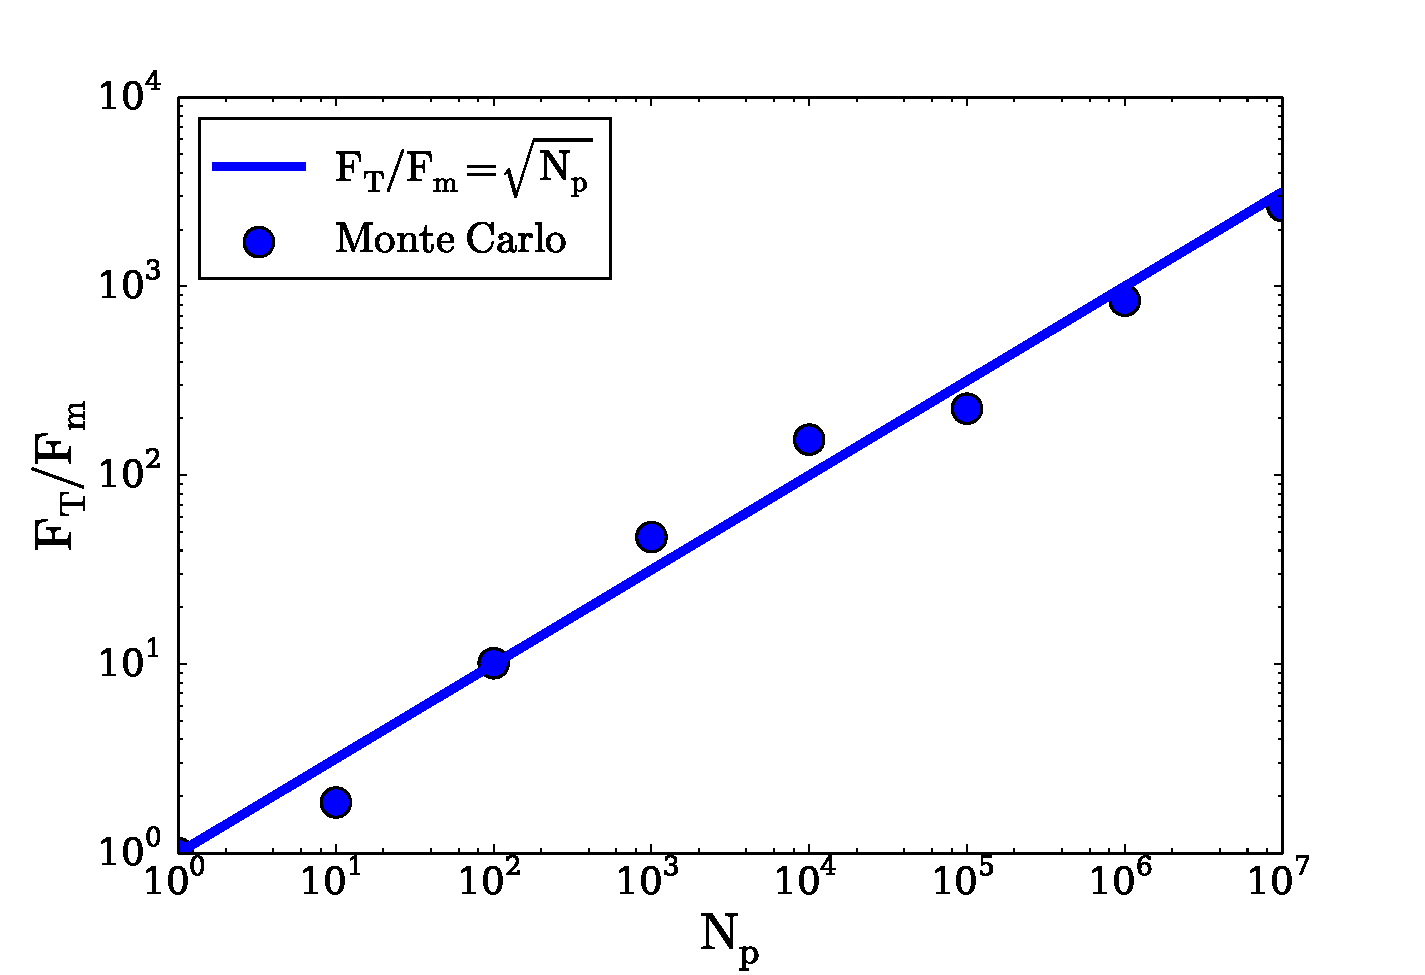
\includegraphics[width=0.80\linewidth,angle=0]{spheres_surface.pdf}
\caption{Norm of the total force per unit mass, $F_{T}$, produced by a
  distribution of $N_p$ point masses randomly distributed over the
  surface of a sphere of radius $R$. The value
  of $F_T$ is  computed at the center of the sphere and is  expressed
  as a multiple  of the force per unit mass produced by a  single
  point mass located  at a distance $R$ from the
  center. \label{fig:sphere_surface}}. 
\end{center}
\end{figure}


\begin{figure}
\begin{center}
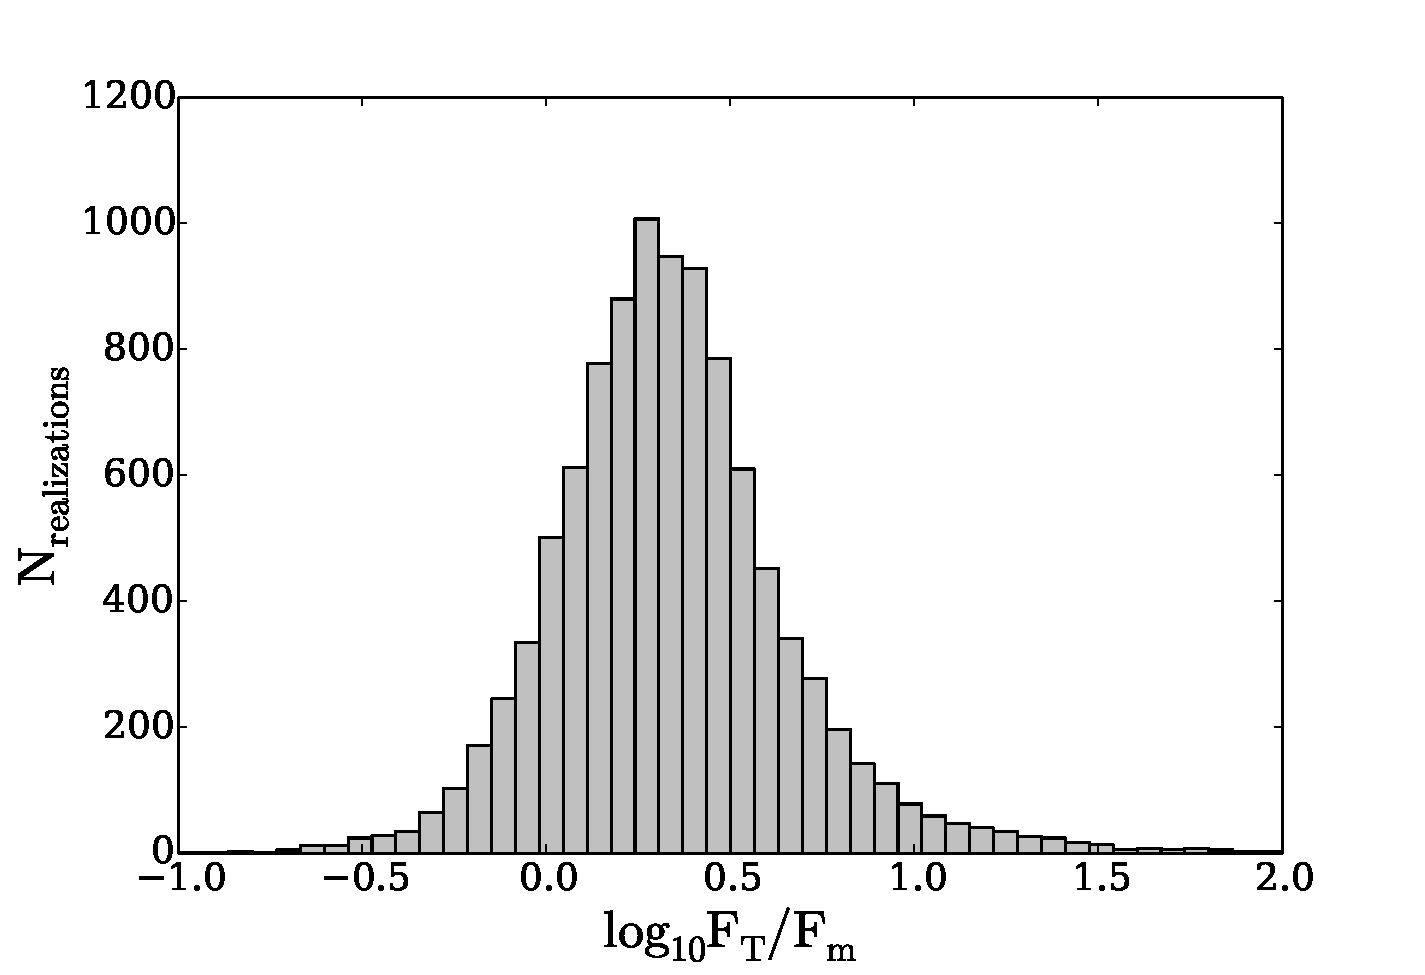
\includegraphics[width=0.8\linewidth,angle=0]{spheres_bulk.pdf}
\caption{\label{fig:sphere_bulk} Frequency of the norm of the total
  force per unit mass produced by a set of identical $N_p$ particles
  homogeneously distributed inside a sphere of radius $R$. This
  corresponds to $10^4$ different realizations of $N_p=10^4$
  particles. The values of $F_T$ is normalized to the force per unit
  mass produced by a single particle located at a distance $R_s$ from
  the center equal to the average interparticle
  separation. \label{fig:sphere_surface}.}  
\end{center}
\end{figure}




\begin{figure}
\begin{center}
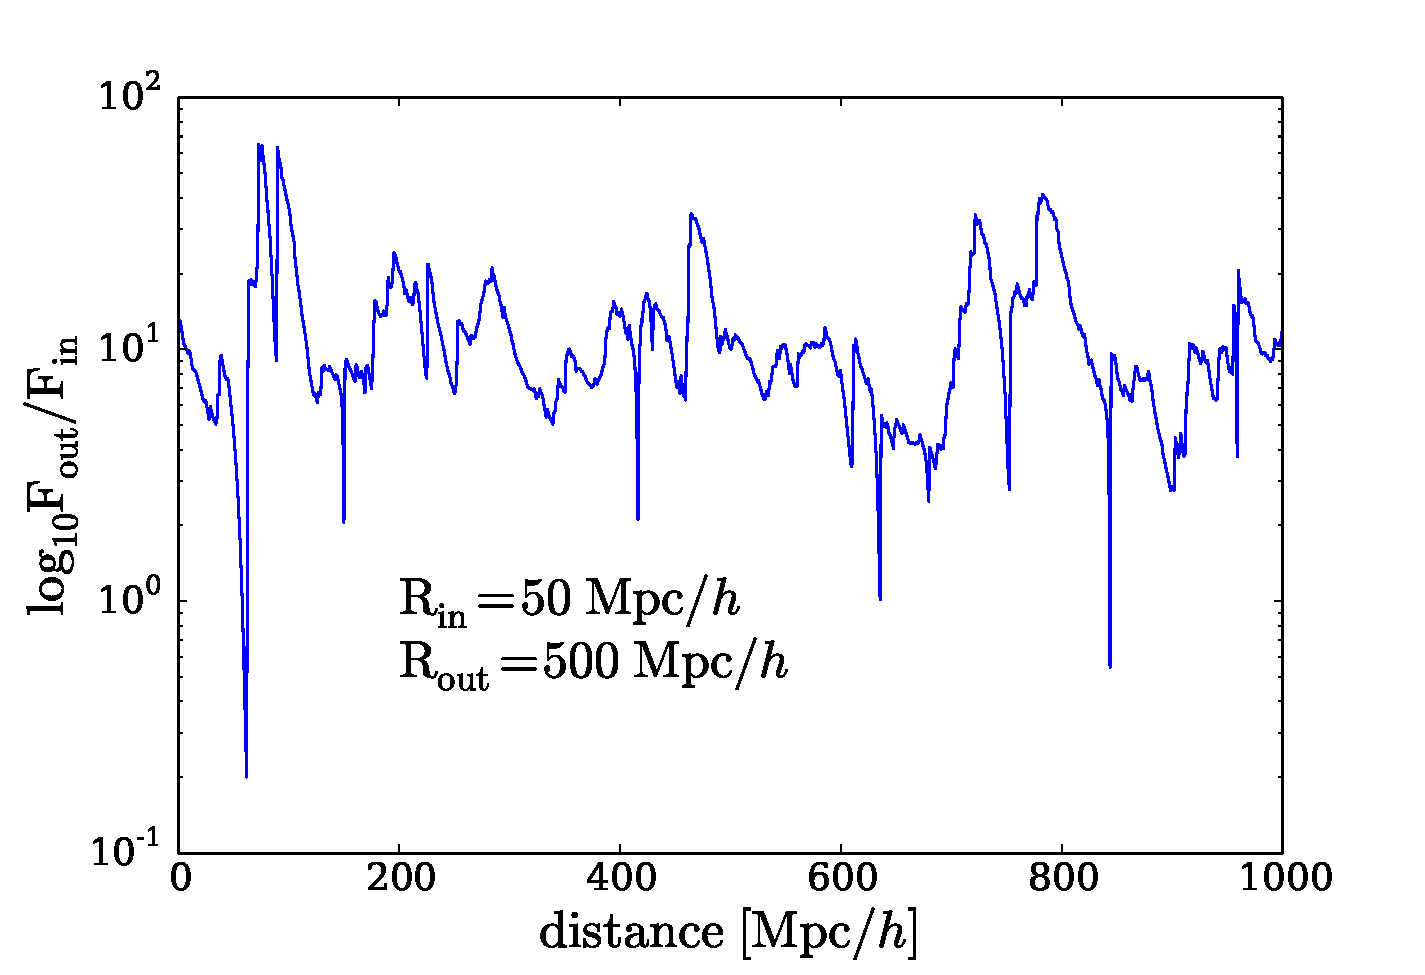
\includegraphics[width=0.8\linewidth,angle=0]{trace_nbody_200_1000.pdf}
\caption{\label{fig:trace_nbody}. Forces produced by dark matter halos in a
simulation along a linear path through the cosmological volume. The
curve presents the ratio between the force produced by all halos
within a spherical shell of halos with radial distances $50\hMpc
<R<500\hMpc$ to the force produced by halos inside 
a sphere of $R<50\hMpc$. }
\end{center}
\end{figure}



\begin{figure}
\begin{center}
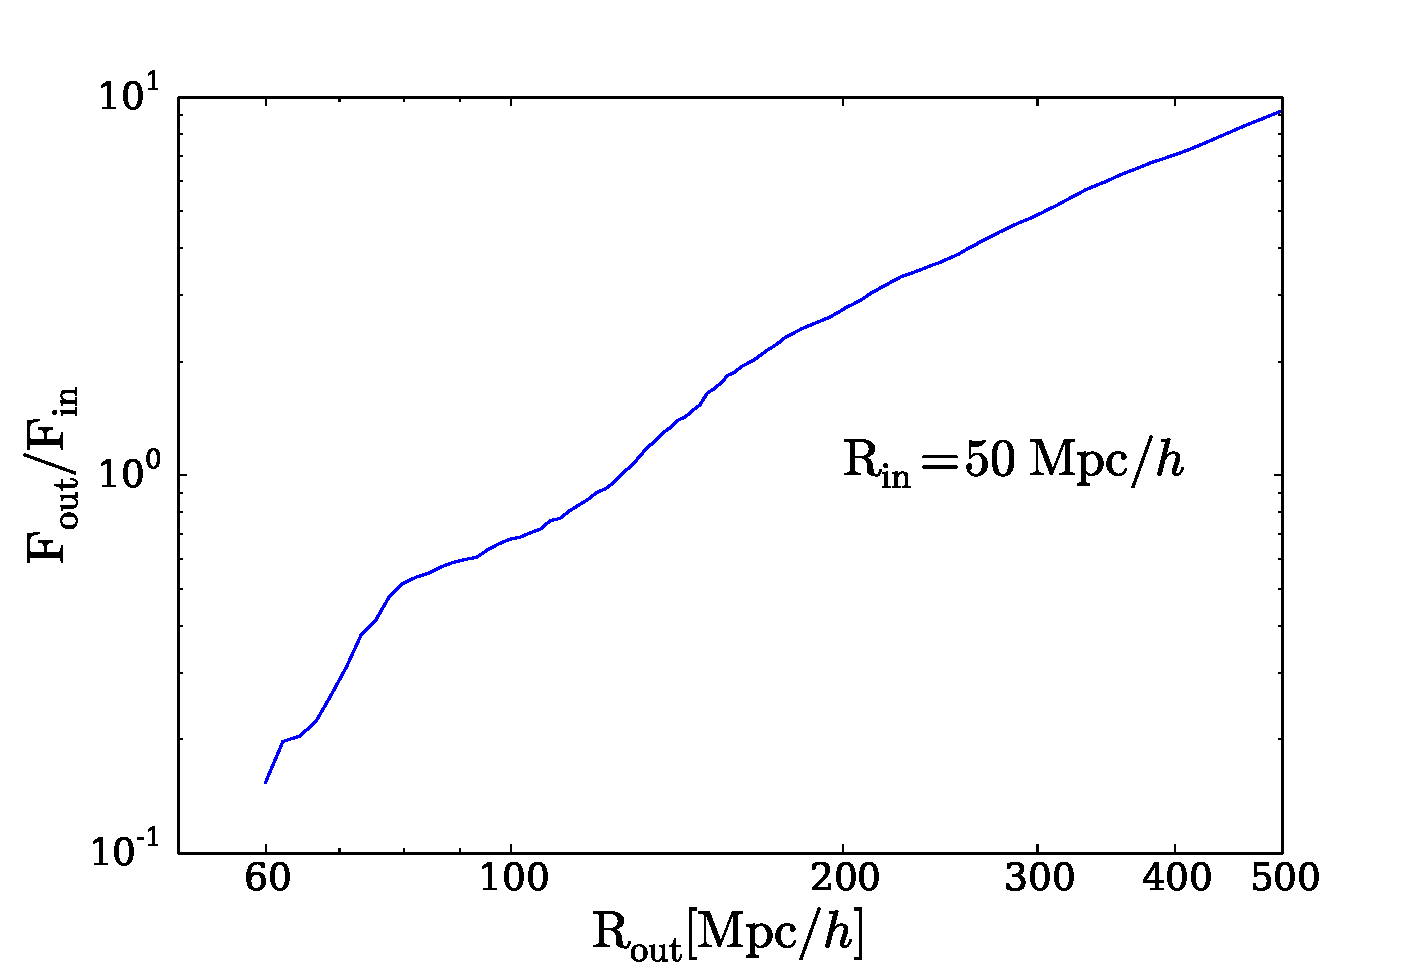
\includegraphics[width=0.8\linewidth,angle=0]{spheres_nbody_radius_200_1000.pdf}
\caption{\label{fig:spheres_radius}. Growth of the total gravitational
  force over ten random dark matter halos in a simulation. Each curve
  presents the between the forces by all halos within a spherical shell with
   radial distances $50\hMpc < R < R_{\rm out}$ to the force produced
   by halos within a sphere of radius $R<50\hMpc$. }  
\end{center}
\end{figure}



\begin{figure}
\begin{center}
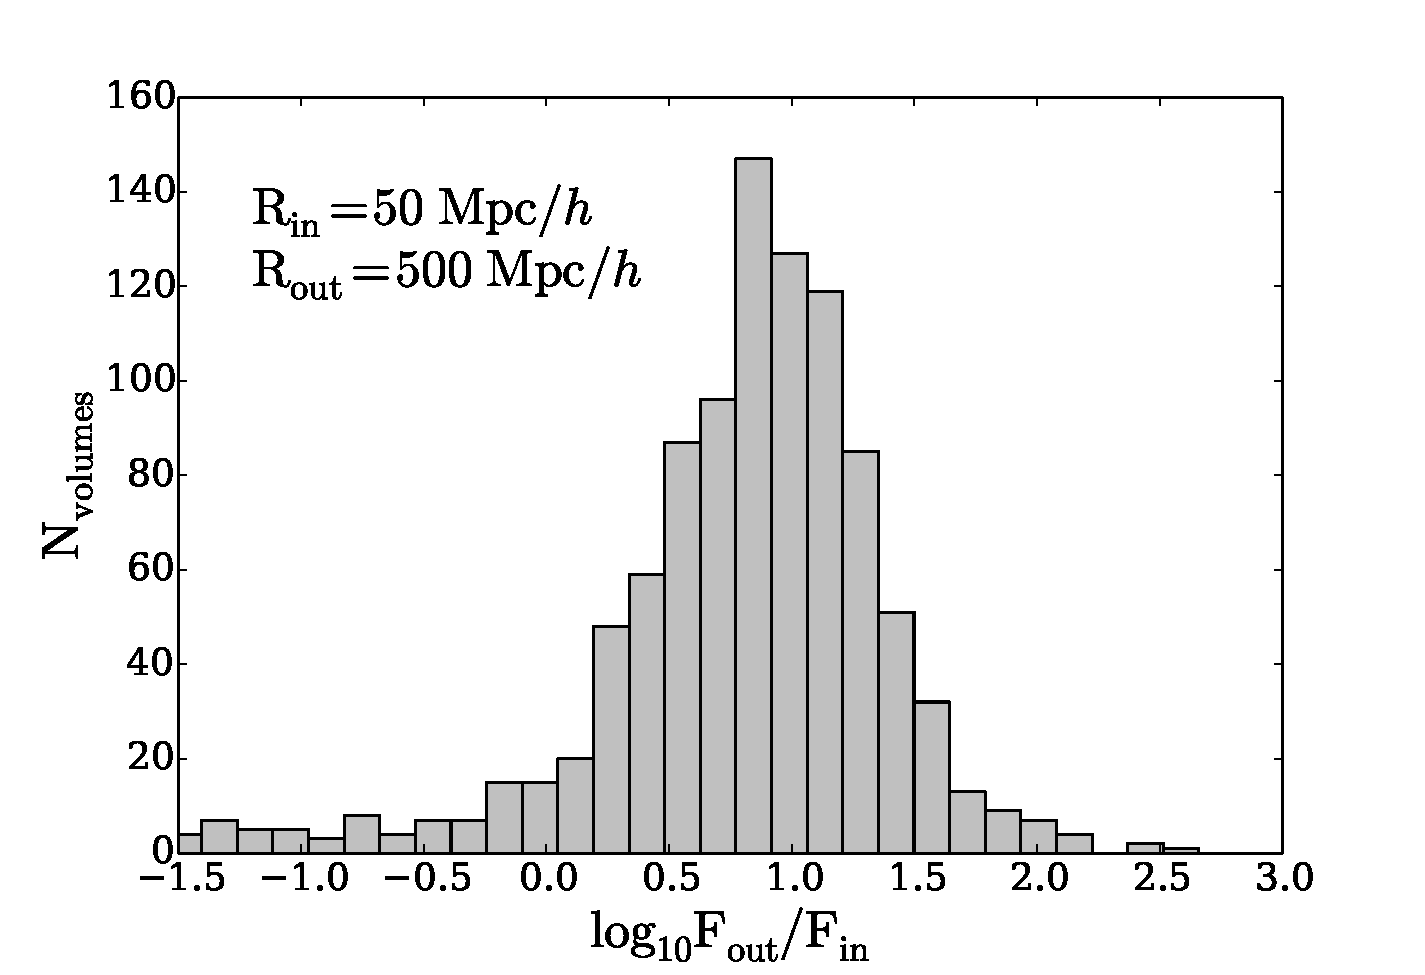
\includegraphics[width=0.8\linewidth,angle=0]{spheres_nbody_200_1000.pdf}
\caption{\label{fig:spheres_nbody} Frequency of the force ratio between
  the halos inside a spherical shell with radial distances $50\hMpc <
  R < 500\hMpc$ and halos within a sphere of radius $R<50\hMpc$. The forces
  are measured at the positions of $1000$ dark matter halos randomly
  selected in the simulated volume.}
\end{center}
\end{figure}



\bibliographystyle{unsrt}
\bibliography{references} 




\end{document}
